\documentclass[]{article}
\usepackage{lmodern}
\usepackage{amssymb,amsmath}
\usepackage{ifxetex,ifluatex}
\usepackage{fixltx2e} % provides \textsubscript
\ifnum 0\ifxetex 1\fi\ifluatex 1\fi=0 % if pdftex
  \usepackage[T1]{fontenc}
  \usepackage[utf8]{inputenc}
\else % if luatex or xelatex
  \ifxetex
    \usepackage{mathspec}
  \else
    \usepackage{fontspec}
  \fi
  \defaultfontfeatures{Ligatures=TeX,Scale=MatchLowercase}
\fi
% use upquote if available, for straight quotes in verbatim environments
\IfFileExists{upquote.sty}{\usepackage{upquote}}{}
% use microtype if available
\IfFileExists{microtype.sty}{%
\usepackage{microtype}
\UseMicrotypeSet[protrusion]{basicmath} % disable protrusion for tt fonts
}{}
\usepackage[margin=1in]{geometry}
\usepackage{hyperref}
\hypersetup{unicode=true,
            pdftitle={R Notebook},
            pdfborder={0 0 0},
            breaklinks=true}
\urlstyle{same}  % don't use monospace font for urls
\usepackage{color}
\usepackage{fancyvrb}
\newcommand{\VerbBar}{|}
\newcommand{\VERB}{\Verb[commandchars=\\\{\}]}
\DefineVerbatimEnvironment{Highlighting}{Verbatim}{commandchars=\\\{\}}
% Add ',fontsize=\small' for more characters per line
\usepackage{framed}
\definecolor{shadecolor}{RGB}{248,248,248}
\newenvironment{Shaded}{\begin{snugshade}}{\end{snugshade}}
\newcommand{\AlertTok}[1]{\textcolor[rgb]{0.94,0.16,0.16}{#1}}
\newcommand{\AnnotationTok}[1]{\textcolor[rgb]{0.56,0.35,0.01}{\textbf{\textit{#1}}}}
\newcommand{\AttributeTok}[1]{\textcolor[rgb]{0.77,0.63,0.00}{#1}}
\newcommand{\BaseNTok}[1]{\textcolor[rgb]{0.00,0.00,0.81}{#1}}
\newcommand{\BuiltInTok}[1]{#1}
\newcommand{\CharTok}[1]{\textcolor[rgb]{0.31,0.60,0.02}{#1}}
\newcommand{\CommentTok}[1]{\textcolor[rgb]{0.56,0.35,0.01}{\textit{#1}}}
\newcommand{\CommentVarTok}[1]{\textcolor[rgb]{0.56,0.35,0.01}{\textbf{\textit{#1}}}}
\newcommand{\ConstantTok}[1]{\textcolor[rgb]{0.00,0.00,0.00}{#1}}
\newcommand{\ControlFlowTok}[1]{\textcolor[rgb]{0.13,0.29,0.53}{\textbf{#1}}}
\newcommand{\DataTypeTok}[1]{\textcolor[rgb]{0.13,0.29,0.53}{#1}}
\newcommand{\DecValTok}[1]{\textcolor[rgb]{0.00,0.00,0.81}{#1}}
\newcommand{\DocumentationTok}[1]{\textcolor[rgb]{0.56,0.35,0.01}{\textbf{\textit{#1}}}}
\newcommand{\ErrorTok}[1]{\textcolor[rgb]{0.64,0.00,0.00}{\textbf{#1}}}
\newcommand{\ExtensionTok}[1]{#1}
\newcommand{\FloatTok}[1]{\textcolor[rgb]{0.00,0.00,0.81}{#1}}
\newcommand{\FunctionTok}[1]{\textcolor[rgb]{0.00,0.00,0.00}{#1}}
\newcommand{\ImportTok}[1]{#1}
\newcommand{\InformationTok}[1]{\textcolor[rgb]{0.56,0.35,0.01}{\textbf{\textit{#1}}}}
\newcommand{\KeywordTok}[1]{\textcolor[rgb]{0.13,0.29,0.53}{\textbf{#1}}}
\newcommand{\NormalTok}[1]{#1}
\newcommand{\OperatorTok}[1]{\textcolor[rgb]{0.81,0.36,0.00}{\textbf{#1}}}
\newcommand{\OtherTok}[1]{\textcolor[rgb]{0.56,0.35,0.01}{#1}}
\newcommand{\PreprocessorTok}[1]{\textcolor[rgb]{0.56,0.35,0.01}{\textit{#1}}}
\newcommand{\RegionMarkerTok}[1]{#1}
\newcommand{\SpecialCharTok}[1]{\textcolor[rgb]{0.00,0.00,0.00}{#1}}
\newcommand{\SpecialStringTok}[1]{\textcolor[rgb]{0.31,0.60,0.02}{#1}}
\newcommand{\StringTok}[1]{\textcolor[rgb]{0.31,0.60,0.02}{#1}}
\newcommand{\VariableTok}[1]{\textcolor[rgb]{0.00,0.00,0.00}{#1}}
\newcommand{\VerbatimStringTok}[1]{\textcolor[rgb]{0.31,0.60,0.02}{#1}}
\newcommand{\WarningTok}[1]{\textcolor[rgb]{0.56,0.35,0.01}{\textbf{\textit{#1}}}}
\usepackage{graphicx,grffile}
\makeatletter
\def\maxwidth{\ifdim\Gin@nat@width>\linewidth\linewidth\else\Gin@nat@width\fi}
\def\maxheight{\ifdim\Gin@nat@height>\textheight\textheight\else\Gin@nat@height\fi}
\makeatother
% Scale images if necessary, so that they will not overflow the page
% margins by default, and it is still possible to overwrite the defaults
% using explicit options in \includegraphics[width, height, ...]{}
\setkeys{Gin}{width=\maxwidth,height=\maxheight,keepaspectratio}
\IfFileExists{parskip.sty}{%
\usepackage{parskip}
}{% else
\setlength{\parindent}{0pt}
\setlength{\parskip}{6pt plus 2pt minus 1pt}
}
\setlength{\emergencystretch}{3em}  % prevent overfull lines
\providecommand{\tightlist}{%
  \setlength{\itemsep}{0pt}\setlength{\parskip}{0pt}}
\setcounter{secnumdepth}{0}
% Redefines (sub)paragraphs to behave more like sections
\ifx\paragraph\undefined\else
\let\oldparagraph\paragraph
\renewcommand{\paragraph}[1]{\oldparagraph{#1}\mbox{}}
\fi
\ifx\subparagraph\undefined\else
\let\oldsubparagraph\subparagraph
\renewcommand{\subparagraph}[1]{\oldsubparagraph{#1}\mbox{}}
\fi

%%% Use protect on footnotes to avoid problems with footnotes in titles
\let\rmarkdownfootnote\footnote%
\def\footnote{\protect\rmarkdownfootnote}

%%% Change title format to be more compact
\usepackage{titling}

% Create subtitle command for use in maketitle
\providecommand{\subtitle}[1]{
  \posttitle{
    \begin{center}\large#1\end{center}
    }
}

\setlength{\droptitle}{-2em}

  \title{R Notebook}
    \pretitle{\vspace{\droptitle}\centering\huge}
  \posttitle{\par}
    \author{}
    \preauthor{}\postauthor{}
    \date{}
    \predate{}\postdate{}
  

\begin{document}
\maketitle

\hypertarget{making-a-shape-from-a-gene}{%
\section{Making a shape from a gene}\label{making-a-shape-from-a-gene}}

OK, let's develop a gene, following the paper. First thing we'll do is
make a shape from a single expression of it.

There is much unsaid in the paper. I'm presuming that the position is
updated as the seed grows. It is unclear where the position ends up as
the tabletop grows at the moment. But the best way to figure it out is
to try it!

\hypertarget{making-the-first-shape}{%
\section{Making the first shape}\label{making-the-first-shape}}

Here, we interpret a single gene and build the stl file to represent the
shape

\begin{Shaded}
\begin{Highlighting}[]
\KeywordTok{source}\NormalTok{(}\StringTok{"../shapevol1/R/sgene.R"}\NormalTok{)}
\KeywordTok{source}\NormalTok{(}\StringTok{"../shapevol1/R/genetostl.R"}\NormalTok{)}
\NormalTok{gene3 <-}\StringTok{ }\KeywordTok{sgene}\NormalTok{(}\StringTok{"DirectionZ"}\NormalTok{,          }\DecValTok{1}\NormalTok{,}\DataTypeTok{status =}\NormalTok{ T,}\DataTypeTok{start=}\FloatTok{0.0}\NormalTok{,}\DataTypeTok{stop=}\FloatTok{0.45}\NormalTok{,}\DataTypeTok{dom=}\DecValTok{1}\NormalTok{)}
\NormalTok{gene4 <-}\StringTok{ }\KeywordTok{sgene}\NormalTok{(}\StringTok{"Cross section"}\NormalTok{,}\StringTok{"Square"}\NormalTok{,}\DataTypeTok{status =}\NormalTok{ T,}\DataTypeTok{start=}\FloatTok{0.0}\NormalTok{,}\DataTypeTok{stop=}\FloatTok{1.5}\NormalTok{,}\DataTypeTok{dom=}\DecValTok{1}\NormalTok{)}
\NormalTok{gene5 <-}\StringTok{ }\KeywordTok{sgene}\NormalTok{(}\StringTok{"Length"}\NormalTok{,            }\FloatTok{0.5}\NormalTok{,}\DataTypeTok{status =}\NormalTok{ T,}\DataTypeTok{start=}\FloatTok{0.0}\NormalTok{,}\DataTypeTok{stop=}\FloatTok{1.5}\NormalTok{,}\DataTypeTok{dom=}\DecValTok{1}\NormalTok{)}
\NormalTok{gene6 <-}\StringTok{ }\KeywordTok{sgene}\NormalTok{(}\StringTok{"Diameter"}\NormalTok{,          }\FloatTok{0.2}\NormalTok{,}\DataTypeTok{status =}\NormalTok{ T,}\DataTypeTok{start=}\FloatTok{0.0}\NormalTok{,}\DataTypeTok{stop=}\FloatTok{1.5}\NormalTok{,}\DataTypeTok{dom=}\DecValTok{1}\NormalTok{)}

\NormalTok{group1 <-}\StringTok{ }\KeywordTok{rbind}\NormalTok{(gene3,gene4,gene5,gene6)}

\KeywordTok{genetostlfile}\NormalTok{(}\StringTok{"~/Desktop/stl/shape1.stl"}\NormalTok{,group1,}\DataTypeTok{runlim=}\DecValTok{1}\NormalTok{)}
\end{Highlighting}
\end{Shaded}

\begin{verbatim}
## writing stl file to ~/Desktop/stl/shape1.stl
\end{verbatim}

\begin{verbatim}
## Iteration 0, position = 0.00,0.00,0.00
\end{verbatim}

\begin{verbatim}
## Cross section is Square
\end{verbatim}

\begin{verbatim}
## Length is 0.50
\end{verbatim}

\begin{verbatim}
## DIA,  ds has 1 rows
\end{verbatim}

\begin{verbatim}
## STST, ds has 1 rows
\end{verbatim}

\begin{verbatim}
## DOM,  ds has 1 rows
\end{verbatim}

\begin{verbatim}
## Diameter is 0.20
\end{verbatim}

\begin{verbatim}
## Found 1 direction genes
\end{verbatim}

\begin{verbatim}
## Found 1 nonzero direction genes, direction is DirectionZ
\end{verbatim}

\begin{verbatim}
## Active Direction is Z
\end{verbatim}

\begin{verbatim}
## Reached DirectionZ stop
\end{verbatim}

\begin{verbatim}
## Running is 0, iterations = 1, runlim = 1
\end{verbatim}

The STL file can be loaded into blender to give the following shape:

\begin{figure}
\centering
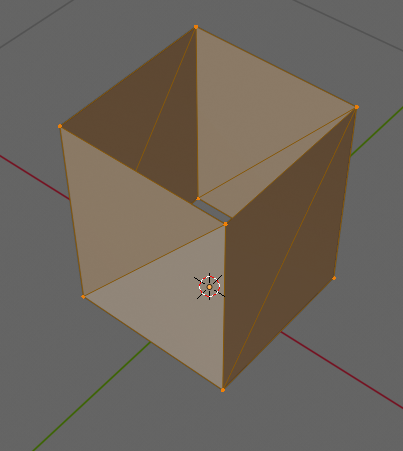
\includegraphics{blender_gene1.png}
\caption{alt text}
\end{figure}

Note that we aren't spending too much time on getting things like wall
thickness right here because we are mainly interested in exploring how
these seed grammars work under evolution. What's missing from the above
is the iterative interpretation of the seed gene. Let's look at how this
works:

\begin{enumerate}
\def\labelenumi{\arabic{enumi}.}
\tightlist
\item
  The current shape is interpreted from the status,start,stop and
  dominance components of each gene, and the current position of the
  growth.
\item
  If a shape is available

  \begin{enumerate}
  \def\labelenumii{\arabic{enumii}.}
  \tightlist
  \item
    The shape is rendered (or ``grown'')
  \item
    The position is updated
  \item
    Return to the top of the loop
  \end{enumerate}
\item
  Otherwise terminate
\end{enumerate}

\hypertarget{shapes-in-other-directions}{%
\subsection{Shapes in other
directions}\label{shapes-in-other-directions}}

Let's make sure we can grow on the X and Y axis also:

\begin{Shaded}
\begin{Highlighting}[]
\KeywordTok{source}\NormalTok{(}\StringTok{"../shapevol1/R/sgene.R"}\NormalTok{)}
\KeywordTok{source}\NormalTok{(}\StringTok{"../shapevol1/R/genetostl.R"}\NormalTok{)}
\NormalTok{gene3 <-}\StringTok{ }\KeywordTok{sgene}\NormalTok{(}\StringTok{"DirectionX"}\NormalTok{,          }\DecValTok{1}\NormalTok{,}\DataTypeTok{status =}\NormalTok{ T,}\DataTypeTok{start=}\FloatTok{0.0}\NormalTok{,}\DataTypeTok{stop=}\FloatTok{0.7}\NormalTok{,}\DataTypeTok{dom=}\DecValTok{1}\NormalTok{)}
\NormalTok{gene4 <-}\StringTok{ }\KeywordTok{sgene}\NormalTok{(}\StringTok{"Cross section"}\NormalTok{,}\StringTok{"Square"}\NormalTok{,}\DataTypeTok{status =}\NormalTok{ T,}\DataTypeTok{start=}\FloatTok{0.0}\NormalTok{,}\DataTypeTok{stop=}\FloatTok{1.5}\NormalTok{,}\DataTypeTok{dom=}\DecValTok{1}\NormalTok{)}
\NormalTok{gene5 <-}\StringTok{ }\KeywordTok{sgene}\NormalTok{(}\StringTok{"Length"}\NormalTok{,            }\FloatTok{0.75}\NormalTok{,}\DataTypeTok{status =}\NormalTok{ T,}\DataTypeTok{start=}\FloatTok{0.0}\NormalTok{,}\DataTypeTok{stop=}\FloatTok{1.5}\NormalTok{,}\DataTypeTok{dom=}\DecValTok{1}\NormalTok{)}
\NormalTok{gene6 <-}\StringTok{ }\KeywordTok{sgene}\NormalTok{(}\StringTok{"Diameter"}\NormalTok{,          }\FloatTok{0.2}\NormalTok{,}\DataTypeTok{status =}\NormalTok{ T,}\DataTypeTok{start=}\FloatTok{0.0}\NormalTok{,}\DataTypeTok{stop=}\FloatTok{1.5}\NormalTok{,}\DataTypeTok{dom=}\DecValTok{1}\NormalTok{)}

\NormalTok{group1 <-}\StringTok{ }\KeywordTok{rbind}\NormalTok{(gene3,gene4,gene5,gene6)}

\KeywordTok{genetostlfile}\NormalTok{(}\StringTok{"~/Desktop/stl/shape1X.stl"}\NormalTok{,group1,}\DataTypeTok{runlim=}\DecValTok{1}\NormalTok{)}
\end{Highlighting}
\end{Shaded}

\begin{verbatim}
## writing stl file to ~/Desktop/stl/shape1X.stl
\end{verbatim}

\begin{verbatim}
## Iteration 0, position = 0.00,0.00,0.00
\end{verbatim}

\begin{verbatim}
## Cross section is Square
\end{verbatim}

\begin{verbatim}
## Length is 0.75
\end{verbatim}

\begin{verbatim}
## DIA,  ds has 1 rows
\end{verbatim}

\begin{verbatim}
## STST, ds has 1 rows
\end{verbatim}

\begin{verbatim}
## DOM,  ds has 1 rows
\end{verbatim}

\begin{verbatim}
## Diameter is 0.20
\end{verbatim}

\begin{verbatim}
## Found 1 direction genes
\end{verbatim}

\begin{verbatim}
## Found 1 nonzero direction genes, direction is DirectionX
\end{verbatim}

\begin{verbatim}
## Active Direction is X
\end{verbatim}

\begin{verbatim}
## Reached DirectionX stop
\end{verbatim}

\begin{verbatim}
## Running is 0, iterations = 1, runlim = 1
\end{verbatim}

\begin{Shaded}
\begin{Highlighting}[]
\KeywordTok{source}\NormalTok{(}\StringTok{"../shapevol1/R/sgene.R"}\NormalTok{)}
\KeywordTok{source}\NormalTok{(}\StringTok{"../shapevol1/R/genetostl.R"}\NormalTok{)}
\NormalTok{gene3 <-}\StringTok{ }\KeywordTok{sgene}\NormalTok{(}\StringTok{"DirectionY"}\NormalTok{,          }\DecValTok{1}\NormalTok{,}\DataTypeTok{status =}\NormalTok{ T,}\DataTypeTok{start=}\FloatTok{0.0}\NormalTok{,}\DataTypeTok{stop=}\FloatTok{0.7}\NormalTok{,}\DataTypeTok{dom=}\DecValTok{1}\NormalTok{)}
\NormalTok{gene4 <-}\StringTok{ }\KeywordTok{sgene}\NormalTok{(}\StringTok{"Cross section"}\NormalTok{,}\StringTok{"Square"}\NormalTok{,}\DataTypeTok{status =}\NormalTok{ T,}\DataTypeTok{start=}\FloatTok{0.0}\NormalTok{,}\DataTypeTok{stop=}\FloatTok{1.5}\NormalTok{,}\DataTypeTok{dom=}\DecValTok{1}\NormalTok{)}
\NormalTok{gene5 <-}\StringTok{ }\KeywordTok{sgene}\NormalTok{(}\StringTok{"Length"}\NormalTok{,            }\FloatTok{0.75}\NormalTok{,}\DataTypeTok{status =}\NormalTok{ T,}\DataTypeTok{start=}\FloatTok{0.0}\NormalTok{,}\DataTypeTok{stop=}\FloatTok{1.5}\NormalTok{,}\DataTypeTok{dom=}\DecValTok{1}\NormalTok{)}
\NormalTok{gene6 <-}\StringTok{ }\KeywordTok{sgene}\NormalTok{(}\StringTok{"Diameter"}\NormalTok{,          }\FloatTok{0.2}\NormalTok{,}\DataTypeTok{status =}\NormalTok{ T,}\DataTypeTok{start=}\FloatTok{0.0}\NormalTok{,}\DataTypeTok{stop=}\FloatTok{1.5}\NormalTok{,}\DataTypeTok{dom=}\DecValTok{1}\NormalTok{)}

\NormalTok{group1 <-}\StringTok{ }\KeywordTok{rbind}\NormalTok{(gene3,gene4,gene5,gene6)}

\KeywordTok{genetostlfile}\NormalTok{(}\StringTok{"~/Desktop/stl/shape1Y.stl"}\NormalTok{,group1,}\DataTypeTok{runlim=}\DecValTok{1}\NormalTok{)}
\end{Highlighting}
\end{Shaded}

\begin{verbatim}
## writing stl file to ~/Desktop/stl/shape1Y.stl
\end{verbatim}

\begin{verbatim}
## Iteration 0, position = 0.00,0.00,0.00
\end{verbatim}

\begin{verbatim}
## Cross section is Square
\end{verbatim}

\begin{verbatim}
## Length is 0.75
\end{verbatim}

\begin{verbatim}
## DIA,  ds has 1 rows
\end{verbatim}

\begin{verbatim}
## STST, ds has 1 rows
\end{verbatim}

\begin{verbatim}
## DOM,  ds has 1 rows
\end{verbatim}

\begin{verbatim}
## Diameter is 0.20
\end{verbatim}

\begin{verbatim}
## Found 1 direction genes
\end{verbatim}

\begin{verbatim}
## Found 1 nonzero direction genes, direction is DirectionY
\end{verbatim}

\begin{verbatim}
## Active Direction is Y
\end{verbatim}

\begin{verbatim}
## Reached DirectionY stop
\end{verbatim}

\begin{verbatim}
## Running is 0, iterations = 1, runlim = 1
\end{verbatim}

\hypertarget{growing-seed-1}{%
\section{Growing seed 1}\label{growing-seed-1}}

Based on the above, we can grow the seed:

\begin{Shaded}
\begin{Highlighting}[]
\KeywordTok{source}\NormalTok{(}\StringTok{"../shapevol1/R/sgene.R"}\NormalTok{)}
\KeywordTok{source}\NormalTok{(}\StringTok{"../shapevol1/R/genetostl.R"}\NormalTok{)}
\NormalTok{gene1 <-}\StringTok{ }\KeywordTok{sgene}\NormalTok{(}\StringTok{"DirectionX"}\NormalTok{,          }\DecValTok{0}\NormalTok{,}\DataTypeTok{status =}\NormalTok{ T,}\DataTypeTok{start=}\FloatTok{0.0}\NormalTok{,}\DataTypeTok{stop=}\FloatTok{1.5}\NormalTok{,}\DataTypeTok{dom=}\DecValTok{1}\NormalTok{)}
\NormalTok{gene2 <-}\StringTok{ }\KeywordTok{sgene}\NormalTok{(}\StringTok{"DirectionY"}\NormalTok{,          }\DecValTok{0}\NormalTok{,}\DataTypeTok{status =}\NormalTok{ T,}\DataTypeTok{start=}\FloatTok{0.0}\NormalTok{,}\DataTypeTok{stop=}\FloatTok{1.5}\NormalTok{,}\DataTypeTok{dom=}\DecValTok{1}\NormalTok{)}
\NormalTok{gene3 <-}\StringTok{ }\KeywordTok{sgene}\NormalTok{(}\StringTok{"DirectionZ"}\NormalTok{,          }\DecValTok{1}\NormalTok{,}\DataTypeTok{status =}\NormalTok{ T,}\DataTypeTok{start=}\FloatTok{0.0}\NormalTok{,}\DataTypeTok{stop=}\FloatTok{1.5}\NormalTok{,}\DataTypeTok{dom=}\DecValTok{1}\NormalTok{)}
\NormalTok{gene4 <-}\StringTok{ }\KeywordTok{sgene}\NormalTok{(}\StringTok{"Cross section"}\NormalTok{,}\StringTok{"Square"}\NormalTok{,}\DataTypeTok{status =}\NormalTok{ T,}\DataTypeTok{start=}\FloatTok{0.0}\NormalTok{,}\DataTypeTok{stop=}\FloatTok{1.5}\NormalTok{,}\DataTypeTok{dom=}\DecValTok{1}\NormalTok{)}
\NormalTok{gene5 <-}\StringTok{ }\KeywordTok{sgene}\NormalTok{(}\StringTok{"Length"}\NormalTok{,            }\FloatTok{0.5}\NormalTok{,}\DataTypeTok{status =}\NormalTok{ T,}\DataTypeTok{start=}\FloatTok{0.0}\NormalTok{,}\DataTypeTok{stop=}\FloatTok{1.5}\NormalTok{,}\DataTypeTok{dom=}\DecValTok{1}\NormalTok{)}
\NormalTok{gene6 <-}\StringTok{ }\KeywordTok{sgene}\NormalTok{(}\StringTok{"Diameter"}\NormalTok{,          }\FloatTok{0.2}\NormalTok{,}\DataTypeTok{status =}\NormalTok{ T,}\DataTypeTok{start=}\FloatTok{0.0}\NormalTok{,}\DataTypeTok{stop=}\FloatTok{1.5}\NormalTok{,}\DataTypeTok{dom=}\DecValTok{1}\NormalTok{)}

\NormalTok{group1 <-}\StringTok{ }\KeywordTok{rbind}\NormalTok{(gene1,gene2,gene3,gene4,gene5,gene6)}

\KeywordTok{genetostlfile}\NormalTok{   (}\StringTok{"~/Desktop/stl/gene1.stl"}\NormalTok{,group1,}\DataTypeTok{runlim=}\DecValTok{10}\NormalTok{)}
\end{Highlighting}
\end{Shaded}

\begin{verbatim}
## writing stl file to ~/Desktop/stl/gene1.stl
\end{verbatim}

\begin{verbatim}
## Iteration 0, position = 0.00,0.00,0.00
\end{verbatim}

\begin{verbatim}
## Cross section is Square
\end{verbatim}

\begin{verbatim}
## Length is 0.50
\end{verbatim}

\begin{verbatim}
## DIA,  ds has 1 rows
\end{verbatim}

\begin{verbatim}
## STST, ds has 1 rows
\end{verbatim}

\begin{verbatim}
## DOM,  ds has 1 rows
\end{verbatim}

\begin{verbatim}
## Diameter is 0.20
\end{verbatim}

\begin{verbatim}
## Found 3 direction genes
\end{verbatim}

\begin{verbatim}
## Found 1 nonzero direction genes, direction is DirectionZ
\end{verbatim}

\begin{verbatim}
## Active Direction is Z
\end{verbatim}

\begin{verbatim}
## Running is 1, iterations = 1, runlim = 10
\end{verbatim}

\begin{verbatim}
## Iteration 1, position = 0.00,0.00,0.50
\end{verbatim}

\begin{verbatim}
## Cross section is Square
\end{verbatim}

\begin{verbatim}
## Length is 0.50
\end{verbatim}

\begin{verbatim}
## DIA,  ds has 1 rows
\end{verbatim}

\begin{verbatim}
## STST, ds has 1 rows
\end{verbatim}

\begin{verbatim}
## DOM,  ds has 1 rows
\end{verbatim}

\begin{verbatim}
## Diameter is 0.20
\end{verbatim}

\begin{verbatim}
## Found 3 direction genes
\end{verbatim}

\begin{verbatim}
## Found 1 nonzero direction genes, direction is DirectionZ
\end{verbatim}

\begin{verbatim}
## Active Direction is Z
\end{verbatim}

\begin{verbatim}
## Running is 1, iterations = 2, runlim = 10
\end{verbatim}

\begin{verbatim}
## Iteration 2, position = 0.00,0.00,1.00
\end{verbatim}

\begin{verbatim}
## Cross section is Square
\end{verbatim}

\begin{verbatim}
## Length is 0.50
\end{verbatim}

\begin{verbatim}
## DIA,  ds has 1 rows
\end{verbatim}

\begin{verbatim}
## STST, ds has 1 rows
\end{verbatim}

\begin{verbatim}
## DOM,  ds has 1 rows
\end{verbatim}

\begin{verbatim}
## Diameter is 0.20
\end{verbatim}

\begin{verbatim}
## Found 3 direction genes
\end{verbatim}

\begin{verbatim}
## Found 1 nonzero direction genes, direction is DirectionZ
\end{verbatim}

\begin{verbatim}
## Active Direction is Z
\end{verbatim}

\begin{verbatim}
## Running is 1, iterations = 3, runlim = 10
\end{verbatim}

\begin{verbatim}
## Iteration 3, position = 0.00,0.00,1.50
\end{verbatim}

\begin{verbatim}
## Cross section is Square
\end{verbatim}

\begin{verbatim}
## Length is 0.50
\end{verbatim}

\begin{verbatim}
## DIA,  ds has 1 rows
\end{verbatim}

\begin{verbatim}
## STST, ds has 1 rows
\end{verbatim}

\begin{verbatim}
## DOM,  ds has 1 rows
\end{verbatim}

\begin{verbatim}
## Diameter is 0.20
\end{verbatim}

\begin{verbatim}
## Found 3 direction genes
\end{verbatim}

\begin{verbatim}
## Found 1 nonzero direction genes, direction is DirectionZ
\end{verbatim}

\begin{verbatim}
## Active Direction is Z
\end{verbatim}

\begin{verbatim}
## Reached DirectionZ stop
\end{verbatim}

\begin{verbatim}
## Running is 0, iterations = 4, runlim = 10
\end{verbatim}

This gives output as

\begin{figure}
\centering
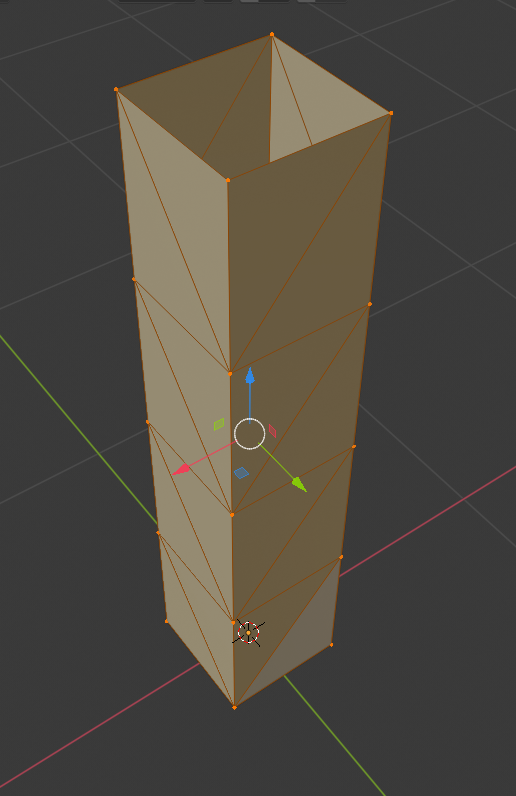
\includegraphics{blender_seed1.png}
\caption{alt text}
\end{figure}

\hypertarget{growing-seed-2}{%
\subsection{Growing seed 2}\label{growing-seed-2}}

Based on the above, we can grow the seed now and check the dominance for
switching between genes. The original paper had the following two genes
to illustrate dominance:

\begin{verbatim}
gene4 = [Cross section, Circle, 1, 0.0, 1.5, 0]
gene7 = [Cross section, Square, 1, 0.0, 0.5, 1] 
\end{verbatim}

Here the cross section changes from shape to square. The \texttt{start}
position is the same for both genes, but the \texttt{stop} position
changes: Gene 7 stops at position 0.5 and gene4 stops at 1.5. Where both
genes are in range, between 0.0 and 0.5, the dominance of gene7 means
this one is expressed.

The original paper highlights the hierarchy of processing as follows:

\begin{enumerate}
\def\labelenumi{\arabic{enumi}.}
\tightlist
\item
  \textbf{ACTIVE} - the gene must be active to have an effect on the
  current iteration. It is not clear how the active status changes while
  the seed is grown
\item
  \textbf{START / STOP} - these refer to the spatial range in which the
  gene takes effect. At present, this is assumed to be \emph{absolute}
  position. Note also it isn't clear which XYZ direction the spatial
  range refers to. I guess we can assume that the value has to be within
  the range of the \emph{current} direction, but this may be problematic
  if more than one direction is specified.
\item
  \textbf{DOMINANCE} - if multiple genes are still active for a
  particular trait, then the trait with the highest dominance value will
  be used. Note that the domiance value must be unique - which will make
  it harder to evolve since we'll have to do a permutation of available
  values, not a mutation.
\end{enumerate}

Below we emulate this idea, but we'll use the diameter of the gene to
show the change, since circular cross sections are difficult to write in
STL:

\begin{Shaded}
\begin{Highlighting}[]
\KeywordTok{source}\NormalTok{(}\StringTok{"../shapevol1/R/sgene.R"}\NormalTok{)}
\KeywordTok{source}\NormalTok{(}\StringTok{"../shapevol1/R/genetostl.R"}\NormalTok{)}
\NormalTok{gene1 <-}\StringTok{ }\KeywordTok{sgene}\NormalTok{(}\StringTok{"DirectionX"}\NormalTok{,          }\DecValTok{0}\NormalTok{,}\DataTypeTok{status =}\NormalTok{ T,}\DataTypeTok{start=}\FloatTok{0.0}\NormalTok{,}\DataTypeTok{stop=}\FloatTok{1.5}\NormalTok{,}\DataTypeTok{dom=}\DecValTok{1}\NormalTok{)}
\NormalTok{gene2 <-}\StringTok{ }\KeywordTok{sgene}\NormalTok{(}\StringTok{"DirectionY"}\NormalTok{,          }\DecValTok{0}\NormalTok{,}\DataTypeTok{status =}\NormalTok{ T,}\DataTypeTok{start=}\FloatTok{0.0}\NormalTok{,}\DataTypeTok{stop=}\FloatTok{1.5}\NormalTok{,}\DataTypeTok{dom=}\DecValTok{1}\NormalTok{)}
\NormalTok{gene3 <-}\StringTok{ }\KeywordTok{sgene}\NormalTok{(}\StringTok{"DirectionZ"}\NormalTok{,          }\DecValTok{1}\NormalTok{,}\DataTypeTok{status =}\NormalTok{ T,}\DataTypeTok{start=}\FloatTok{0.0}\NormalTok{,}\DataTypeTok{stop=}\FloatTok{1.5}\NormalTok{,}\DataTypeTok{dom=}\DecValTok{1}\NormalTok{)}
\NormalTok{gene4 <-}\StringTok{ }\KeywordTok{sgene}\NormalTok{(}\StringTok{"Cross section"}\NormalTok{,}\StringTok{"Square"}\NormalTok{,}\DataTypeTok{status =}\NormalTok{ T,}\DataTypeTok{start=}\FloatTok{0.0}\NormalTok{,}\DataTypeTok{stop=}\FloatTok{1.5}\NormalTok{,}\DataTypeTok{dom=}\DecValTok{1}\NormalTok{)}
\NormalTok{gene5 <-}\StringTok{ }\KeywordTok{sgene}\NormalTok{(}\StringTok{"Length"}\NormalTok{,            }\FloatTok{0.5}\NormalTok{,}\DataTypeTok{status =}\NormalTok{ T,}\DataTypeTok{start=}\FloatTok{0.0}\NormalTok{,}\DataTypeTok{stop=}\FloatTok{1.5}\NormalTok{,}\DataTypeTok{dom=}\DecValTok{1}\NormalTok{)}
\NormalTok{gene6 <-}\StringTok{ }\KeywordTok{sgene}\NormalTok{(}\StringTok{"Diameter"}\NormalTok{,          }\FloatTok{0.3}\NormalTok{,}\DataTypeTok{status =}\NormalTok{ T,}\DataTypeTok{start=}\FloatTok{0.0}\NormalTok{,}\DataTypeTok{stop=}\FloatTok{1.5}\NormalTok{,}\DataTypeTok{dom=}\DecValTok{0}\NormalTok{)}
\NormalTok{gene7 <-}\StringTok{ }\KeywordTok{sgene}\NormalTok{(}\StringTok{"Diameter"}\NormalTok{,          }\FloatTok{0.2}\NormalTok{,}\DataTypeTok{status =}\NormalTok{ T,}\DataTypeTok{start=}\FloatTok{0.0}\NormalTok{,}\DataTypeTok{stop=}\FloatTok{0.5}\NormalTok{,}\DataTypeTok{dom=}\DecValTok{1}\NormalTok{)}

\NormalTok{group1 <-}\StringTok{ }\KeywordTok{rbind}\NormalTok{(gene1,gene2,gene3,gene4,gene5,gene6,gene7)}

\KeywordTok{genetostlfile}\NormalTok{   (}\StringTok{"~/Desktop/stl/gene2.stl"}\NormalTok{,group1,}\DataTypeTok{runlim=}\DecValTok{10}\NormalTok{)}
\end{Highlighting}
\end{Shaded}

\begin{verbatim}
## writing stl file to ~/Desktop/stl/gene2.stl
\end{verbatim}

\begin{verbatim}
## Iteration 0, position = 0.00,0.00,0.00
\end{verbatim}

\begin{verbatim}
## Cross section is Square
\end{verbatim}

\begin{verbatim}
## Length is 0.50
\end{verbatim}

\begin{verbatim}
## DIA,  ds has 2 rows
\end{verbatim}

\begin{verbatim}
## STST, ds has 2 rows
\end{verbatim}

\begin{verbatim}
## DOM,  ds has 1 rows
\end{verbatim}

\begin{verbatim}
## Diameter is 0.20
\end{verbatim}

\begin{verbatim}
## Found 3 direction genes
\end{verbatim}

\begin{verbatim}
## Found 1 nonzero direction genes, direction is DirectionZ
\end{verbatim}

\begin{verbatim}
## Active Direction is Z
\end{verbatim}

\begin{verbatim}
## Running is 1, iterations = 1, runlim = 10
\end{verbatim}

\begin{verbatim}
## Iteration 1, position = 0.00,0.00,0.50
\end{verbatim}

\begin{verbatim}
## Cross section is Square
\end{verbatim}

\begin{verbatim}
## Length is 0.50
\end{verbatim}

\begin{verbatim}
## DIA,  ds has 2 rows
\end{verbatim}

\begin{verbatim}
## STST, ds has 2 rows
\end{verbatim}

\begin{verbatim}
## DOM,  ds has 1 rows
\end{verbatim}

\begin{verbatim}
## Diameter is 0.20
\end{verbatim}

\begin{verbatim}
## Found 3 direction genes
\end{verbatim}

\begin{verbatim}
## Found 1 nonzero direction genes, direction is DirectionZ
\end{verbatim}

\begin{verbatim}
## Active Direction is Z
\end{verbatim}

\begin{verbatim}
## Running is 1, iterations = 2, runlim = 10
\end{verbatim}

\begin{verbatim}
## Iteration 2, position = 0.00,0.00,1.00
\end{verbatim}

\begin{verbatim}
## Cross section is Square
\end{verbatim}

\begin{verbatim}
## Length is 0.50
\end{verbatim}

\begin{verbatim}
## DIA,  ds has 2 rows
\end{verbatim}

\begin{verbatim}
## STST, ds has 1 rows
\end{verbatim}

\begin{verbatim}
## DOM,  ds has 1 rows
\end{verbatim}

\begin{verbatim}
## Diameter is 0.30
\end{verbatim}

\begin{verbatim}
## Found 3 direction genes
\end{verbatim}

\begin{verbatim}
## Found 1 nonzero direction genes, direction is DirectionZ
\end{verbatim}

\begin{verbatim}
## Active Direction is Z
\end{verbatim}

\begin{verbatim}
## Running is 1, iterations = 3, runlim = 10
\end{verbatim}

\begin{verbatim}
## Iteration 3, position = 0.00,0.00,1.50
\end{verbatim}

\begin{verbatim}
## Cross section is Square
\end{verbatim}

\begin{verbatim}
## Length is 0.50
\end{verbatim}

\begin{verbatim}
## DIA,  ds has 2 rows
\end{verbatim}

\begin{verbatim}
## STST, ds has 1 rows
\end{verbatim}

\begin{verbatim}
## DOM,  ds has 1 rows
\end{verbatim}

\begin{verbatim}
## Diameter is 0.30
\end{verbatim}

\begin{verbatim}
## Found 3 direction genes
\end{verbatim}

\begin{verbatim}
## Found 1 nonzero direction genes, direction is DirectionZ
\end{verbatim}

\begin{verbatim}
## Active Direction is Z
\end{verbatim}

\begin{verbatim}
## Reached DirectionZ stop
\end{verbatim}

\begin{verbatim}
## Running is 0, iterations = 4, runlim = 10
\end{verbatim}

OK, that worked! result is:

\begin{figure}
\centering
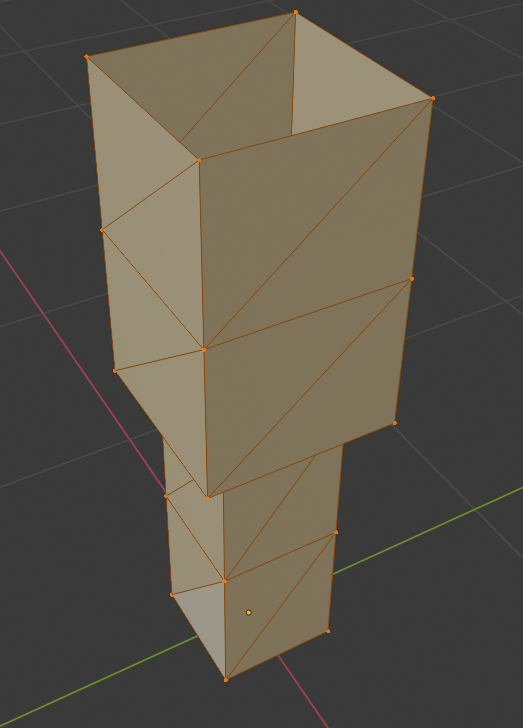
\includegraphics{seed2.png}
\caption{seed 2}
\end{figure}

Now we need to move on to the more complex shape in seed3. This will
involve manipulation of the axis of growth, so we'd better write a new
function for it:

\#Growing seed 3

Let's do this group by group, following figure 4 in the paper:

\begin{Shaded}
\begin{Highlighting}[]
\NormalTok{gene01 <-}\StringTok{ }\KeywordTok{sgene}\NormalTok{(}\StringTok{"Cross section"}\NormalTok{,}\StringTok{"Square"}\NormalTok{,}\DataTypeTok{status =}\NormalTok{ T,}\DataTypeTok{start=}\OperatorTok{-}\DecValTok{40}\NormalTok{,}\DataTypeTok{stop=}\DecValTok{40}\NormalTok{,}\DataTypeTok{dom=}\DecValTok{1}\NormalTok{)}
\NormalTok{gene02 <-}\StringTok{ }\KeywordTok{sgene}\NormalTok{(}\StringTok{"Length"}\NormalTok{,       }\DecValTok{5}\NormalTok{       ,}\DataTypeTok{status =}\NormalTok{ T,}\DataTypeTok{start=}\OperatorTok{-}\DecValTok{40}\NormalTok{,}\DataTypeTok{stop=}\DecValTok{40}\NormalTok{,}\DataTypeTok{dom=}\DecValTok{1}\NormalTok{)}
\NormalTok{gene03 <-}\StringTok{ }\KeywordTok{sgene}\NormalTok{(}\StringTok{"Diameter"}\NormalTok{,     }\DecValTok{2}\NormalTok{       ,}\DataTypeTok{status =}\NormalTok{ T,}\DataTypeTok{start=}\OperatorTok{-}\DecValTok{40}\NormalTok{,}\DataTypeTok{stop=}\DecValTok{40}\NormalTok{,}\DataTypeTok{dom=}\DecValTok{0}\NormalTok{)}
\NormalTok{group1 <-}\StringTok{ }\KeywordTok{rbind}\NormalTok{(gene01,gene02,gene03)}
\end{Highlighting}
\end{Shaded}

At this point, we can't grow a gene as we have no direction information,
but let's now add group 2 and try to grow the resulting seed:

\begin{Shaded}
\begin{Highlighting}[]
\NormalTok{gene04 <-}\StringTok{ }\KeywordTok{sgene}\NormalTok{(}\StringTok{"X_1Z"}\NormalTok{,          }\DecValTok{0}\NormalTok{,}\DataTypeTok{status =}\NormalTok{ T,}\DataTypeTok{start=}\DecValTok{0}\NormalTok{,}\DataTypeTok{stop=}\DecValTok{5}\NormalTok{,}\DataTypeTok{dom=}\DecValTok{1}\NormalTok{)}
\NormalTok{gene05 <-}\StringTok{ }\KeywordTok{sgene}\NormalTok{(}\StringTok{"Y_1Z"}\NormalTok{,          }\DecValTok{0}\NormalTok{,}\DataTypeTok{status =}\NormalTok{ T,}\DataTypeTok{start=}\DecValTok{0}\NormalTok{,}\DataTypeTok{stop=}\DecValTok{5}\NormalTok{,}\DataTypeTok{dom=}\DecValTok{1}\NormalTok{)}
\NormalTok{gene06 <-}\StringTok{ }\KeywordTok{sgene}\NormalTok{(}\StringTok{"Z_1Z"}\NormalTok{,          }\DecValTok{1}\NormalTok{,}\DataTypeTok{status =}\NormalTok{ T,}\DataTypeTok{start=}\DecValTok{0}\NormalTok{,}\DataTypeTok{stop=}\DecValTok{5}\NormalTok{,}\DataTypeTok{dom=}\DecValTok{1}\NormalTok{)}

\NormalTok{gene07 <-}\StringTok{ }\KeywordTok{sgene}\NormalTok{(}\StringTok{"X_1X"}\NormalTok{,          }\DecValTok{0}\NormalTok{,}\DataTypeTok{status =}\NormalTok{ T,}\DataTypeTok{start=}\DecValTok{0}\NormalTok{,}\DataTypeTok{stop=}\DecValTok{1}\NormalTok{,}\DataTypeTok{dom=}\DecValTok{1}\NormalTok{)}
\NormalTok{gene08 <-}\StringTok{ }\KeywordTok{sgene}\NormalTok{(}\StringTok{"Y_1X"}\NormalTok{,          }\DecValTok{0}\NormalTok{,}\DataTypeTok{status =}\NormalTok{ T,}\DataTypeTok{start=}\DecValTok{0}\NormalTok{,}\DataTypeTok{stop=}\DecValTok{1}\NormalTok{,}\DataTypeTok{dom=}\DecValTok{1}\NormalTok{)}
\NormalTok{gene09 <-}\StringTok{ }\KeywordTok{sgene}\NormalTok{(}\StringTok{"Z_1X"}\NormalTok{,          }\DecValTok{1}\NormalTok{,}\DataTypeTok{status =}\NormalTok{ T,}\DataTypeTok{start=}\DecValTok{0}\NormalTok{,}\DataTypeTok{stop=}\DecValTok{1}\NormalTok{,}\DataTypeTok{dom=}\DecValTok{1}\NormalTok{)}

\NormalTok{gene10 <-}\StringTok{ }\KeywordTok{sgene}\NormalTok{(}\StringTok{"X_1Y"}\NormalTok{,          }\DecValTok{0}\NormalTok{,}\DataTypeTok{status =}\NormalTok{ T,}\DataTypeTok{start=}\DecValTok{0}\NormalTok{,}\DataTypeTok{stop=}\DecValTok{1}\NormalTok{,}\DataTypeTok{dom=}\DecValTok{1}\NormalTok{)}
\NormalTok{gene11 <-}\StringTok{ }\KeywordTok{sgene}\NormalTok{(}\StringTok{"Y_1Y"}\NormalTok{,          }\DecValTok{0}\NormalTok{,}\DataTypeTok{status =}\NormalTok{ T,}\DataTypeTok{start=}\DecValTok{0}\NormalTok{,}\DataTypeTok{stop=}\DecValTok{1}\NormalTok{,}\DataTypeTok{dom=}\DecValTok{1}\NormalTok{)}
\NormalTok{gene12 <-}\StringTok{ }\KeywordTok{sgene}\NormalTok{(}\StringTok{"Z_1Y"}\NormalTok{,          }\DecValTok{1}\NormalTok{,}\DataTypeTok{status =}\NormalTok{ T,}\DataTypeTok{start=}\DecValTok{0}\NormalTok{,}\DataTypeTok{stop=}\DecValTok{1}\NormalTok{,}\DataTypeTok{dom=}\DecValTok{1}\NormalTok{)}
\NormalTok{group2 <-}\StringTok{ }\KeywordTok{rbind}\NormalTok{(gene04,gene05,gene06,gene07,gene08,gene09,gene10,gene11,gene12)}
\end{Highlighting}
\end{Shaded}

Some observations: - Genes without reserved names ``Cross section'',
``Length'', ``Diameter'', are direction genes. It's still pretty
difficult to work out \emph{which} direction - here I'm taking the last
letter as an indication (which works with this gene) - seems pointless
having genes for particular directions that \emph{never} have an effect,
but I'm copying the paper to check. - the start and stop values for
dimension attributes clearly pertain to that direction - should the
start/stop directions be passed to other attributes at the point of
adding them to the model? This seems to raise the risk of having missing
attributes unless we are careful - evolving the models will expose this
- These genes are all of attribute 1 or 0 - multiples of the ``Len''
gene to get a unit length of 5

Let's try and grow this seed and see what happens. We'll develop a new
function now because it's going to be a bumpy ride!

\begin{Shaded}
\begin{Highlighting}[]
\KeywordTok{require}\NormalTok{(stringr)}
\end{Highlighting}
\end{Shaded}

\begin{verbatim}
## Loading required package: stringr
\end{verbatim}

\begin{Shaded}
\begin{Highlighting}[]
\KeywordTok{source}\NormalTok{(}\StringTok{"../shapevol1/R/sgene.R"}\NormalTok{)}
\KeywordTok{source}\NormalTok{(}\StringTok{"../shapevol1/R/genetostl.R"}\NormalTok{)}
\KeywordTok{genetostlfile2}\NormalTok{   (}\StringTok{"~/Desktop/stl/seed3s3.stl"}\NormalTok{,}\KeywordTok{rbind}\NormalTok{(group1,group2),}\DataTypeTok{runlim=}\DecValTok{10}\NormalTok{)}
\end{Highlighting}
\end{Shaded}

\begin{verbatim}
## writing stl file to ~/Desktop/stl/seed3s3.stl
\end{verbatim}

\begin{verbatim}
## Iteration 0, position = 0.00,0.00,0.00
\end{verbatim}

\begin{verbatim}
## Cross section is Square
\end{verbatim}

\begin{verbatim}
## Multiple Lengths!
\end{verbatim}

\begin{verbatim}
## Length is 5.00
\end{verbatim}

\begin{verbatim}
## DIA,  ds has 1 rows
\end{verbatim}

\begin{verbatim}
## STST, ds has 1 rows
\end{verbatim}

\begin{verbatim}
## DOM,  ds has 1 rows
\end{verbatim}

\begin{verbatim}
## Diameter is 2.00
\end{verbatim}

\begin{verbatim}
## Found 3 X direction genes
\end{verbatim}

\begin{verbatim}
## Found 3 Y direction genes
\end{verbatim}

\begin{verbatim}
## Found 3 Z direction genes
\end{verbatim}

\begin{verbatim}
## Found 3 nonzero direction genes, direction is Z_1X
\end{verbatim}

\begin{verbatim}
## Active Direction is X
\end{verbatim}

\begin{verbatim}
## Running is 1, iterations = 1, runlim = 10
\end{verbatim}

\begin{verbatim}
## Iteration 1, position = 5.00,0.00,0.00
\end{verbatim}

\begin{verbatim}
## Cross section is Square
\end{verbatim}

\begin{verbatim}
## Multiple Lengths!
\end{verbatim}

\begin{verbatim}
## Length is 5.00
\end{verbatim}

\begin{verbatim}
## DIA,  ds has 1 rows
\end{verbatim}

\begin{verbatim}
## STST, ds has 1 rows
\end{verbatim}

\begin{verbatim}
## DOM,  ds has 1 rows
\end{verbatim}

\begin{verbatim}
## Diameter is 2.00
\end{verbatim}

\begin{verbatim}
## Found 3 X direction genes
\end{verbatim}

\begin{verbatim}
## Found 3 Y direction genes
\end{verbatim}

\begin{verbatim}
## Found 3 Z direction genes
\end{verbatim}

\begin{verbatim}
## Found 3 nonzero direction genes, direction is Z_1X
\end{verbatim}

\begin{verbatim}
## Active Direction is N
\end{verbatim}

\begin{verbatim}
## Running is 1, iterations = 2, runlim = 10
\end{verbatim}

\begin{verbatim}
## Iteration 2, position = 5.00,0.00,0.00
\end{verbatim}

\begin{verbatim}
## Cross section is Square
\end{verbatim}

\begin{verbatim}
## Multiple Lengths!
\end{verbatim}

\begin{verbatim}
## Length is 5.00
\end{verbatim}

\begin{verbatim}
## DIA,  ds has 1 rows
\end{verbatim}

\begin{verbatim}
## STST, ds has 1 rows
\end{verbatim}

\begin{verbatim}
## DOM,  ds has 1 rows
\end{verbatim}

\begin{verbatim}
## Diameter is 2.00
\end{verbatim}

\begin{verbatim}
## Found 3 X direction genes
\end{verbatim}

\begin{verbatim}
## Found 3 Y direction genes
\end{verbatim}

\begin{verbatim}
## Found 3 Z direction genes
\end{verbatim}

\begin{verbatim}
## Found 3 nonzero direction genes, direction is Z_1X
\end{verbatim}

\begin{verbatim}
## Active Direction is N
\end{verbatim}

\begin{verbatim}
## Running is 1, iterations = 3, runlim = 10
\end{verbatim}

\begin{verbatim}
## Iteration 3, position = 5.00,0.00,0.00
\end{verbatim}

\begin{verbatim}
## Cross section is Square
\end{verbatim}

\begin{verbatim}
## Multiple Lengths!
\end{verbatim}

\begin{verbatim}
## Length is 5.00
\end{verbatim}

\begin{verbatim}
## DIA,  ds has 1 rows
\end{verbatim}

\begin{verbatim}
## STST, ds has 1 rows
\end{verbatim}

\begin{verbatim}
## DOM,  ds has 1 rows
\end{verbatim}

\begin{verbatim}
## Diameter is 2.00
\end{verbatim}

\begin{verbatim}
## Found 3 X direction genes
\end{verbatim}

\begin{verbatim}
## Found 3 Y direction genes
\end{verbatim}

\begin{verbatim}
## Found 3 Z direction genes
\end{verbatim}

\begin{verbatim}
## Found 3 nonzero direction genes, direction is Z_1X
\end{verbatim}

\begin{verbatim}
## Active Direction is N
\end{verbatim}

\begin{verbatim}
## Running is 1, iterations = 4, runlim = 10
\end{verbatim}

\begin{verbatim}
## Iteration 4, position = 5.00,0.00,0.00
\end{verbatim}

\begin{verbatim}
## Cross section is Square
\end{verbatim}

\begin{verbatim}
## Multiple Lengths!
\end{verbatim}

\begin{verbatim}
## Length is 5.00
\end{verbatim}

\begin{verbatim}
## DIA,  ds has 1 rows
\end{verbatim}

\begin{verbatim}
## STST, ds has 1 rows
\end{verbatim}

\begin{verbatim}
## DOM,  ds has 1 rows
\end{verbatim}

\begin{verbatim}
## Diameter is 2.00
\end{verbatim}

\begin{verbatim}
## Found 3 X direction genes
\end{verbatim}

\begin{verbatim}
## Found 3 Y direction genes
\end{verbatim}

\begin{verbatim}
## Found 3 Z direction genes
\end{verbatim}

\begin{verbatim}
## Found 3 nonzero direction genes, direction is Z_1X
\end{verbatim}

\begin{verbatim}
## Active Direction is N
\end{verbatim}

\begin{verbatim}
## Running is 1, iterations = 5, runlim = 10
\end{verbatim}

\begin{verbatim}
## Iteration 5, position = 5.00,0.00,0.00
\end{verbatim}

\begin{verbatim}
## Cross section is Square
\end{verbatim}

\begin{verbatim}
## Multiple Lengths!
\end{verbatim}

\begin{verbatim}
## Length is 5.00
\end{verbatim}

\begin{verbatim}
## DIA,  ds has 1 rows
\end{verbatim}

\begin{verbatim}
## STST, ds has 1 rows
\end{verbatim}

\begin{verbatim}
## DOM,  ds has 1 rows
\end{verbatim}

\begin{verbatim}
## Diameter is 2.00
\end{verbatim}

\begin{verbatim}
## Found 3 X direction genes
\end{verbatim}

\begin{verbatim}
## Found 3 Y direction genes
\end{verbatim}

\begin{verbatim}
## Found 3 Z direction genes
\end{verbatim}

\begin{verbatim}
## Found 3 nonzero direction genes, direction is Z_1X
\end{verbatim}

\begin{verbatim}
## Active Direction is N
\end{verbatim}

\begin{verbatim}
## Running is 1, iterations = 6, runlim = 10
\end{verbatim}

\begin{verbatim}
## Iteration 6, position = 5.00,0.00,0.00
\end{verbatim}

\begin{verbatim}
## Cross section is Square
\end{verbatim}

\begin{verbatim}
## Multiple Lengths!
\end{verbatim}

\begin{verbatim}
## Length is 5.00
\end{verbatim}

\begin{verbatim}
## DIA,  ds has 1 rows
\end{verbatim}

\begin{verbatim}
## STST, ds has 1 rows
\end{verbatim}

\begin{verbatim}
## DOM,  ds has 1 rows
\end{verbatim}

\begin{verbatim}
## Diameter is 2.00
\end{verbatim}

\begin{verbatim}
## Found 3 X direction genes
\end{verbatim}

\begin{verbatim}
## Found 3 Y direction genes
\end{verbatim}

\begin{verbatim}
## Found 3 Z direction genes
\end{verbatim}

\begin{verbatim}
## Found 3 nonzero direction genes, direction is Z_1X
\end{verbatim}

\begin{verbatim}
## Active Direction is N
\end{verbatim}

\begin{verbatim}
## Running is 1, iterations = 7, runlim = 10
\end{verbatim}

\begin{verbatim}
## Iteration 7, position = 5.00,0.00,0.00
\end{verbatim}

\begin{verbatim}
## Cross section is Square
\end{verbatim}

\begin{verbatim}
## Multiple Lengths!
\end{verbatim}

\begin{verbatim}
## Length is 5.00
\end{verbatim}

\begin{verbatim}
## DIA,  ds has 1 rows
\end{verbatim}

\begin{verbatim}
## STST, ds has 1 rows
\end{verbatim}

\begin{verbatim}
## DOM,  ds has 1 rows
\end{verbatim}

\begin{verbatim}
## Diameter is 2.00
\end{verbatim}

\begin{verbatim}
## Found 3 X direction genes
\end{verbatim}

\begin{verbatim}
## Found 3 Y direction genes
\end{verbatim}

\begin{verbatim}
## Found 3 Z direction genes
\end{verbatim}

\begin{verbatim}
## Found 3 nonzero direction genes, direction is Z_1X
\end{verbatim}

\begin{verbatim}
## Active Direction is N
\end{verbatim}

\begin{verbatim}
## Running is 1, iterations = 8, runlim = 10
\end{verbatim}

\begin{verbatim}
## Iteration 8, position = 5.00,0.00,0.00
\end{verbatim}

\begin{verbatim}
## Cross section is Square
\end{verbatim}

\begin{verbatim}
## Multiple Lengths!
\end{verbatim}

\begin{verbatim}
## Length is 5.00
\end{verbatim}

\begin{verbatim}
## DIA,  ds has 1 rows
\end{verbatim}

\begin{verbatim}
## STST, ds has 1 rows
\end{verbatim}

\begin{verbatim}
## DOM,  ds has 1 rows
\end{verbatim}

\begin{verbatim}
## Diameter is 2.00
\end{verbatim}

\begin{verbatim}
## Found 3 X direction genes
\end{verbatim}

\begin{verbatim}
## Found 3 Y direction genes
\end{verbatim}

\begin{verbatim}
## Found 3 Z direction genes
\end{verbatim}

\begin{verbatim}
## Found 3 nonzero direction genes, direction is Z_1X
\end{verbatim}

\begin{verbatim}
## Active Direction is N
\end{verbatim}

\begin{verbatim}
## Running is 1, iterations = 9, runlim = 10
\end{verbatim}

\begin{verbatim}
## Iteration 9, position = 5.00,0.00,0.00
\end{verbatim}

\begin{verbatim}
## Cross section is Square
\end{verbatim}

\begin{verbatim}
## Multiple Lengths!
\end{verbatim}

\begin{verbatim}
## Length is 5.00
\end{verbatim}

\begin{verbatim}
## DIA,  ds has 1 rows
\end{verbatim}

\begin{verbatim}
## STST, ds has 1 rows
\end{verbatim}

\begin{verbatim}
## DOM,  ds has 1 rows
\end{verbatim}

\begin{verbatim}
## Diameter is 2.00
\end{verbatim}

\begin{verbatim}
## Found 3 X direction genes
\end{verbatim}

\begin{verbatim}
## Found 3 Y direction genes
\end{verbatim}

\begin{verbatim}
## Found 3 Z direction genes
\end{verbatim}

\begin{verbatim}
## Found 3 nonzero direction genes, direction is Z_1X
\end{verbatim}

\begin{verbatim}
## Active Direction is N
\end{verbatim}

\begin{verbatim}
## Running is 1, iterations = 10, runlim = 10
\end{verbatim}

\begin{verbatim}
## Iteration 10, position = 5.00,0.00,0.00
\end{verbatim}

\begin{verbatim}
## Cross section is Square
\end{verbatim}

\begin{verbatim}
## Multiple Lengths!
\end{verbatim}

\begin{verbatim}
## Length is 5.00
\end{verbatim}

\begin{verbatim}
## DIA,  ds has 1 rows
\end{verbatim}

\begin{verbatim}
## STST, ds has 1 rows
\end{verbatim}

\begin{verbatim}
## DOM,  ds has 1 rows
\end{verbatim}

\begin{verbatim}
## Diameter is 2.00
\end{verbatim}

\begin{verbatim}
## Found 3 X direction genes
\end{verbatim}

\begin{verbatim}
## Found 3 Y direction genes
\end{verbatim}

\begin{verbatim}
## Found 3 Z direction genes
\end{verbatim}

\begin{verbatim}
## Found 3 nonzero direction genes, direction is Z_1X
\end{verbatim}

\begin{verbatim}
## Active Direction is N
\end{verbatim}

\begin{verbatim}
## Running is 1, iterations = 11, runlim = 10
\end{verbatim}

\begin{verbatim}
## Iteration 11, position = 5.00,0.00,0.00
\end{verbatim}

\begin{verbatim}
## Cross section is Square
\end{verbatim}

\begin{verbatim}
## Multiple Lengths!
\end{verbatim}

\begin{verbatim}
## Length is 5.00
\end{verbatim}

\begin{verbatim}
## DIA,  ds has 1 rows
\end{verbatim}

\begin{verbatim}
## STST, ds has 1 rows
\end{verbatim}

\begin{verbatim}
## DOM,  ds has 1 rows
\end{verbatim}

\begin{verbatim}
## Diameter is 2.00
\end{verbatim}

\begin{verbatim}
## Found 3 X direction genes
\end{verbatim}

\begin{verbatim}
## Found 3 Y direction genes
\end{verbatim}

\begin{verbatim}
## Found 3 Z direction genes
\end{verbatim}

\begin{verbatim}
## Found 3 nonzero direction genes, direction is Z_1X
\end{verbatim}

\begin{verbatim}
## Active Direction is N
\end{verbatim}

\begin{verbatim}
## finished
\end{verbatim}

\begin{verbatim}
## Running is 0, iterations = 12, runlim = 10
\end{verbatim}

It's starting to look like we have to maintain a \emph{list} of
positions and build at each position as we go along. It isn't clear
whether or how these added positions should be removed once added atm.


\end{document}
